%
% differenz.tex
%
% (c) 2021 Prof Dr Andreas Müller, OST Ostschweizer Fachhochschule
%
\documentclass[tikz]{standalone}
\usepackage{times}
\usepackage{amsmath}
\usepackage{txfonts}
\usepackage[utf8]{inputenc}
\usepackage{graphics}
\usetikzlibrary{arrows,intersections,math,calc}
\definecolor{darkred}{rgb}{0.8,0,0}
\usepackage{ifthen}
\begin{document}

\newboolean{showgrid}
\setboolean{showgrid}{false}
\def\breite{6}
\def\hoehe{8}

\begin{tikzpicture}[>=latex,thick]

% Povray Bild
\begin{scope}[yshift=5.5cm]
	\clip (-5.3,-2.9) rectangle (5.3,2.5);
	\node at (0,0) {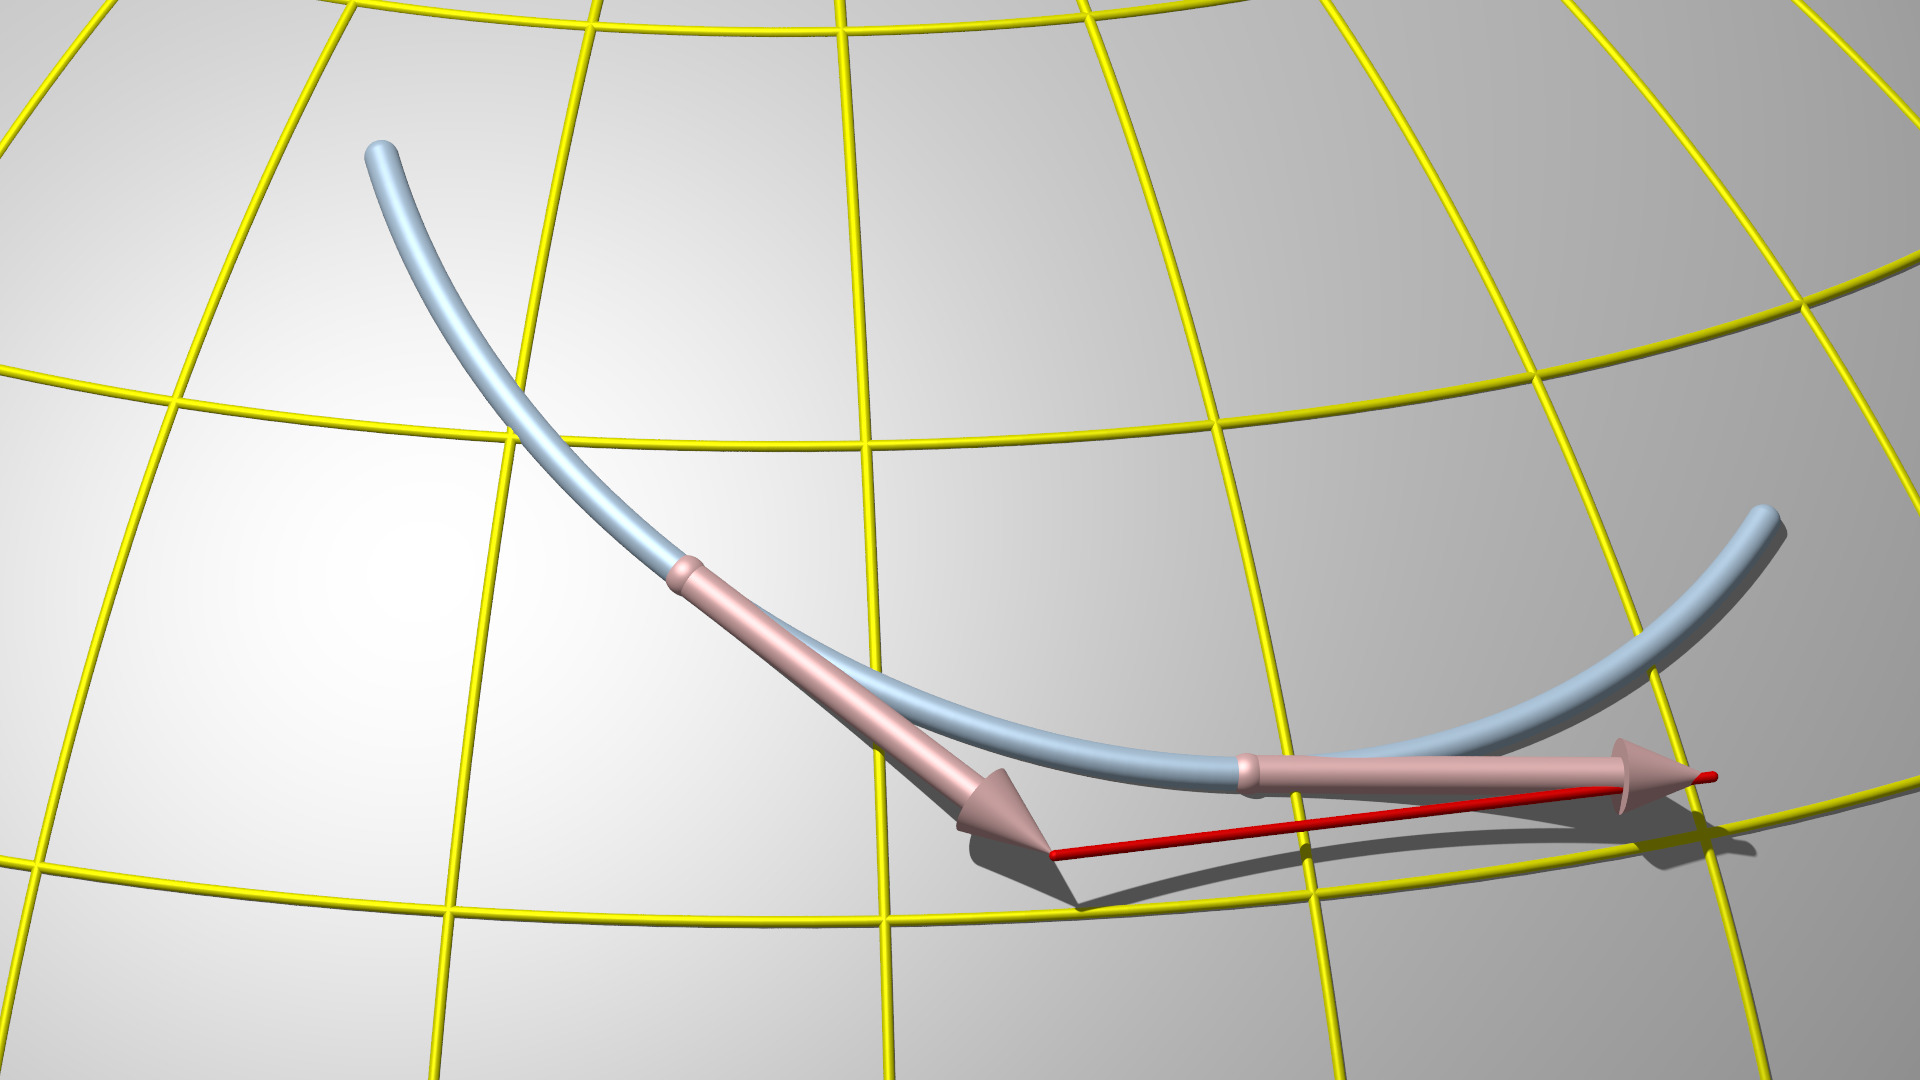
\includegraphics[width=10.6cm]{differenz.jpg}};
	\node at (-1.8,-0.5) {$\gamma(t)$};
	\node at (0.1,-1.9) {$\dot{\gamma}(t)$};
	\node at (1.6,-0.95) {$\gamma(t+\Delta t)$};
	\node at (4,-1.8) {$\dot{\gamma}(t+\Delta t)$};
	\node[color=darkred] at (2.1,-1.8) {?};
	\node at (-4.8,2.1) {(a)\strut};
\end{scope}
\begin{scope}
	\clip (-5.3,-3.0) rectangle (5.3,2.5);
	\node at (0,0) {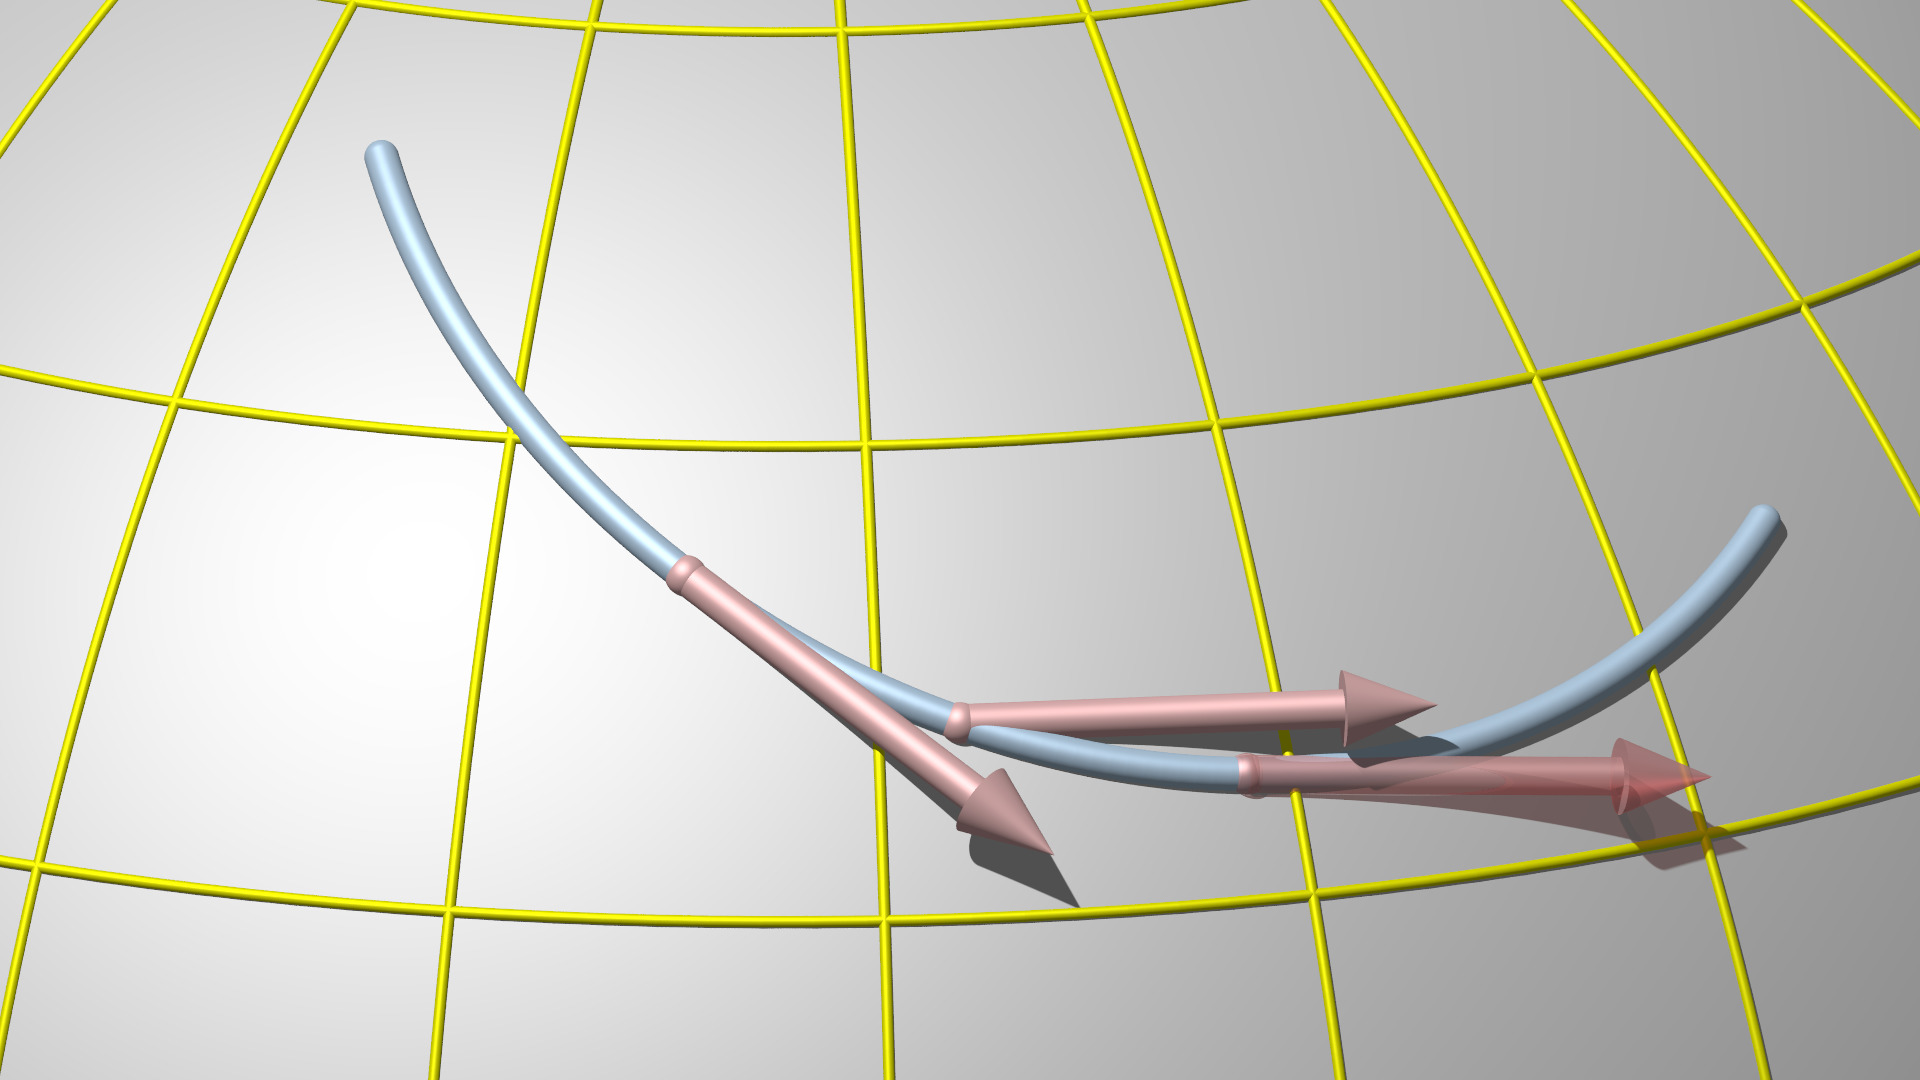
\includegraphics[width=10.6cm]{d06.jpg}};
	\coordinate (A) at (4.1,-1.3);
	\coordinate (B) at (1.1,-0.5);
	\draw[->,color=darkred,opacity=0.7,line width=1.4pt]
		(A) -- ($0.5*(A)+0.5*(B)$);
	\draw[->,color=darkred,opacity=0.7,line width=1.4pt]
		($0.5*(A)+0.5*(B)$) -- (B);
	\node at (-4.8,2.1) {(b)\strut};
\end{scope}
\begin{scope}[yshift=-5.6cm]
	\clip (-5.3,-2.9) rectangle (5.3,2.5);
	\node at (0,0) {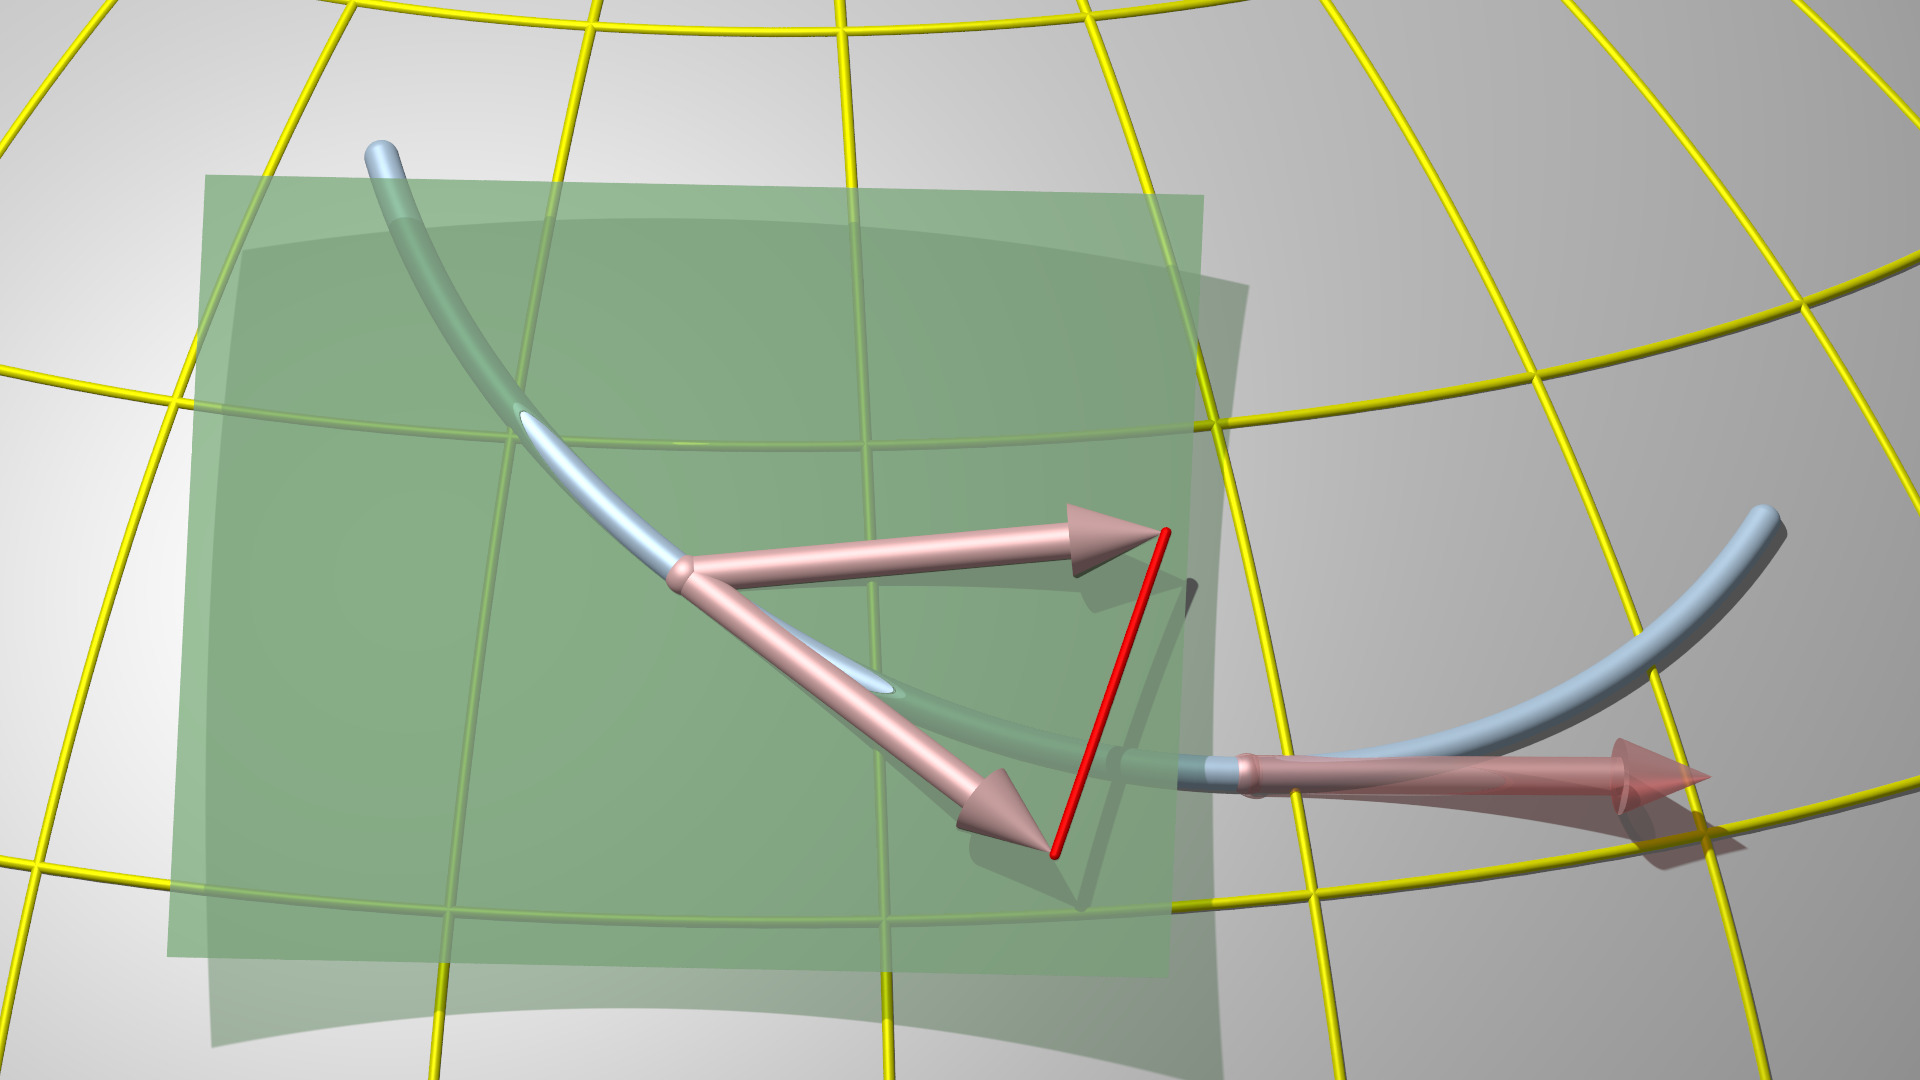
\includegraphics[width=10.6cm]{diffgedreht.jpg}};
	\node at (-1.8,-0.5) {$\gamma(t)$};
	\node at (0.1,-1.9) {$\dot{\gamma}(t)$};
	\node at (0.5,1.5) {$T_{\gamma(t)}M$};
	\node at (-4.8,2.1) {(c)\strut};
\end{scope}

% Gitter
\ifthenelse{\boolean{showgrid}}{
\draw[step=0.1,line width=0.1pt] (-\breite,-\hoehe) grid (\breite, \hoehe);
\draw[step=0.5,line width=0.4pt] (-\breite,-\hoehe) grid (\breite, \hoehe);
\draw                            (-\breite,-\hoehe) grid (\breite, \hoehe);
\fill (0,0) circle[radius=0.05];
}{}

\end{tikzpicture}

\end{document}

